\subsubsection{MSVC}

\RU{Компилируем в}\EN{Compile it in} MSVC 2010:

\lstinputlisting[caption=MSVC 2010: \ttf{}]{patterns/12_FPU/1_simple/MSVC.asm.\LANG}

\RU{\FLD берет 8 байт из стека и загружает их в регистр \ST{0}, автоматически конвертируя во внутренний 
80-битный формат (\IT{extended precision}).}
\EN{\FLD takes 8 bytes from stack and loads the number into the \ST{0} register, automatically converting 
it into the internal 80-bit format (\IT{extended precision}).}

\index{x86!\Instructions!FDIV}
\RU{\FDIV делит содержимое регистра \ST{0} на число, лежащее по адресу \TT{\_\_real@40091eb851eb851f}~--- 
там закодировано значение 3,14. Синтаксис ассемблера не поддерживает подобные числа, 
поэтому мы там видим шестнадцатеричное представление числа 3,14 в формате IEEE 754.}
\EN{\FDIV divides the value in \ST{0} by the number stored at address 
\TT{\_\_real@40091eb851eb851f}~---the value 3.14 is encoded there. 
The assembly syntax doesn't support floating point numbers, so 
what we see here is the hexadecimal representation of 3.14 in 64-bit IEEE 754 format.}

\RU{После выполнения \FDIV в \ST{0} остается \glslink{quotient}{частное}.}
\EN{After the execution of \FDIV \ST{0} holds the \gls{quotient}.}

\index{x86!\Instructions!FDIVP}
\RU{Кстати, есть ещё инструкция \FDIVP, которая делит \ST{1} на \ST{0}, 
выталкивает эти числа из стека и заталкивает результат. 
Если вы знаете язык Forth\FNURLFORTH, то это как раз оно и есть~--- стековая машина\FNURLSTACK.}
\EN{By the way, there is also the \FDIVP instruction, which divides \ST{1} by \ST{0}, 
popping both these values from stack and then pushing the result. 
If you know the Forth language\FNURLFORTH,
you can quickly understand that this is a stack machine\FNURLSTACK.}

\RU{Следующая \FLD заталкивает в стек значение $b$.}
\EN{The subsequent \FLD instruction pushes the value of $b$ into the stack.}

\RU{После этого в \ST{1} перемещается результат деления, а в \ST{0} теперь $b$.}
\EN{After that, the quotient is placed in \ST{1}, and \ST{0} has the value of $b$.}

\index{x86!\Instructions!FMUL}
\RU{Следующий \FMUL умножает $b$ из \ST{0} на значение \TT{\_\_real@4010666666666666}~--- 
там лежит число 4,1~--- и оставляет результат в \ST{0}.}
\EN{The next \FMUL instruction does multiplication: $b$ from \ST{0} is multiplied by by value at 
\TT{\_\_real@4010666666666666} (the numer 4.1 is there) and leaves the result in the \ST{0} register.}

\index{x86!\Instructions!FADDP}
\RU{Самая последняя инструкция \FADDP складывает два значения из вершины стека 
в \ST{1} и затем выталкивает значение, лежащее в \ST{0}. 
Таким образом результат сложения остается на вершине стека в \ST{0}.}
\EN{The last \FADDP instruction adds the two values at top of stack, storing the result in \ST{1} 
and then popping the value of \ST{0}, thereby leaving the result at the top of the stack, in \ST{0}.}

\RU{Функция должна вернуть результат в \ST{0}, так что больше ничего здесь не производится, 
кроме эпилога функции.}
\EN{The function must return its result in the \ST{0} register, 
so there are no any other instructions except the function epilogue after \FADDP.}

\ifdefined\IncludeOlly
\clearpage
\subsubsection{MSVC + \olly}
\index{\olly}

\RU{2 пары 32-битных слов обведены в стеке красным. Каждая пара\EMDASH{}
это числа двойной точности в формате IEEE 754, переданные из \main.}
\EN{2 pairs of 32-bit words are marked by red in the stack. 
Each pair is a double-number in IEEE 754 format and is passed from \main.}
\RU{Видно, как первая \FLD загружает значение 1,2 из стека и помещает в регистр \ST{0}:}
\EN{We see how the first \FLD loads a value ($1.2$) from the stack and puts it into \ST{0}:}

\begin{figure}[H]
\centering
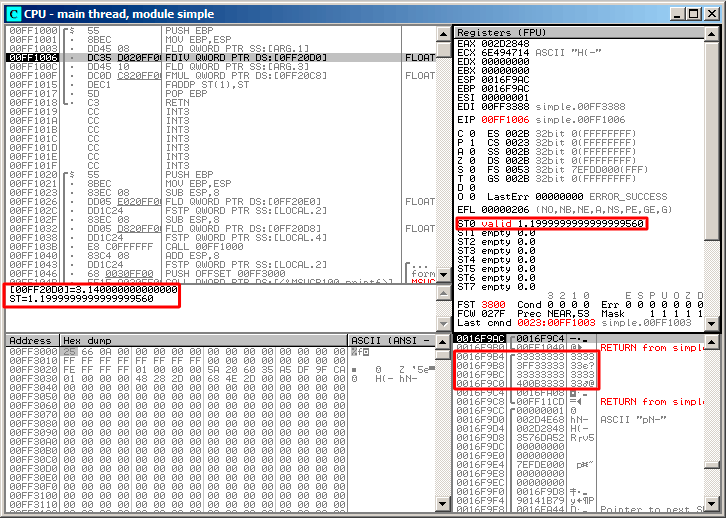
\includegraphics[scale=\FigScale]{patterns/12_FPU/1_simple/olly1.png}
\caption{\olly: \RU{первая \FLD исполнилась}\EN{first \FLD executed}}
\label{fig:FPU_simple_olly_1}
\end{figure}

\RU{Из-за неизбежных ошибок конвертирования числа из 64-битного IEEE 754 в 80-битное (внутреннее в FPU),
мы видим здесь 1,1999\ldots, что очень близко к 1,2.}
\EN{Because of unavoidable conversion errors from 64-bit IEEE 754 floating point to 80-bit
(used internally in the FPU), here we see 1.999\ldots, which is close to 1.2.}
\RU{Прямо сейчас \EIP указывает на следующую инструкцию (\FDIV), загружающую константу двойной точности 
из памяти.}
\EN{\EIP now points to the next instruction (\FDIV), which loads a double-number (a constant)
from memory.}
\RU{Для удобства}\EN{For convenience}, \olly \RU{показывает её значение: 3,14.}\EN{shows its value: 3.14}

\clearpage
\RU{Трассируем дальше}\EN{Let's trace further}. 
\FDIV \RU{исполнилась}\EN{was executed}, \RU{теперь}\EN{now} \ST{0} \RU{содержит 0,382\ldots}\EN{contains 0.382\ldots}
(\gls{quotient}):

\begin{figure}[H]
\centering
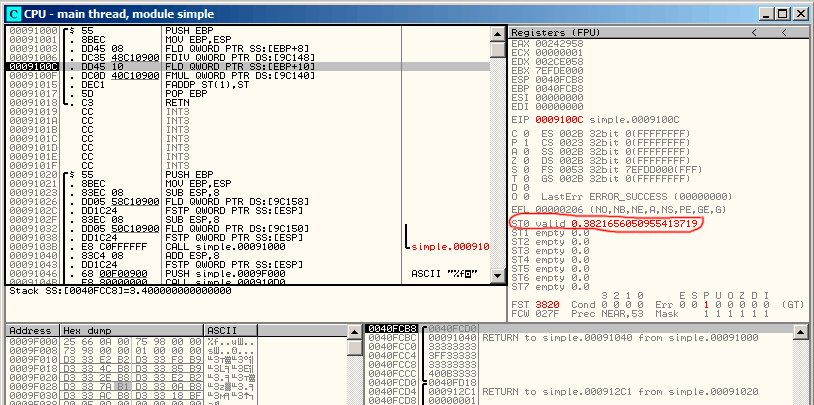
\includegraphics[scale=\FigScale]{patterns/12_FPU/1_simple/olly2.png}
\caption{\olly: \FDIV \RU{исполнилась}\EN{executed}}
\label{fig:FPU_simple_olly_2}
\end{figure}

\clearpage
\RU{Третий шаг}\EN{Third step}: \RU{вторая}\EN{the next} \FLD 
\RU{исполнилась, загрузив в \ST{0} 3,4 (мы видим приближенное число 3,39999\ldots)}
\EN{was executed, loading 3.4 into \ST{0} (here we see the approximate value 3.39999\ldots)}: 

\begin{figure}[H]
\centering
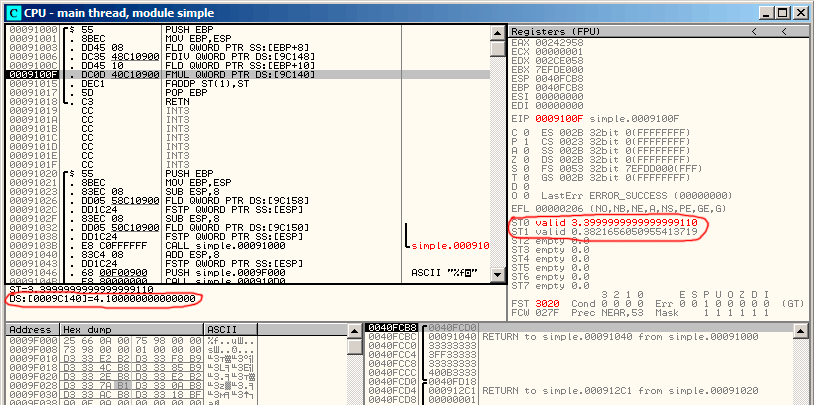
\includegraphics[scale=\FigScale]{patterns/12_FPU/1_simple/olly3.png}
\caption{\olly: \RU{вторая \FLD исполнилась}\EN{second \FLD executed}}
\label{fig:FPU_simple_olly_3}
\end{figure}

\RU{В это время}\EN{At the same time,} \gls{quotient} \IT{\RU{провалилось}\EN{is pushed}} 
\RU{в}\EN{into} \ST{1}.
\RU{\EIP указывает на следующую инструкцию}\EN{Right now, \EIP points to the next
instruction}: \FMUL. 
\RU{Она загружает константу 4,1}\EN{It loads the constant 4.1} \RU{из памяти, так что \olly тоже показывает её здесь}
\EN{from memory, which \olly shows}.

\clearpage
\RU{Затем}\EN{Next}: \FMUL \RU{исполнилась, теперь в \ST{0} произведение}%
\EN{was executed, so now the \gls{product} is in \ST{0}}:

\begin{figure}[H]
\centering
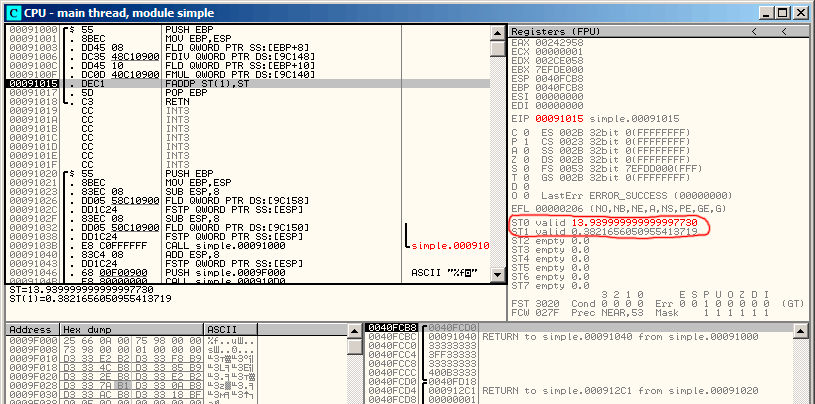
\includegraphics[scale=\FigScale]{patterns/12_FPU/1_simple/olly4.png}
\caption{\olly: \FMUL \RU{исполнилась}\EN{executed}}
\label{fig:FPU_simple_olly_4}
\end{figure}

\clearpage
\RU{Затем}\EN{Next}: \FADDP \RU{исполнилась, теперь в \ST{0} сумма, а \ST{1} очистился}%
\EN{was executed, now the result of the addition is in \ST{0}, and \ST{1} is cleared}:

\begin{figure}[H]
\centering
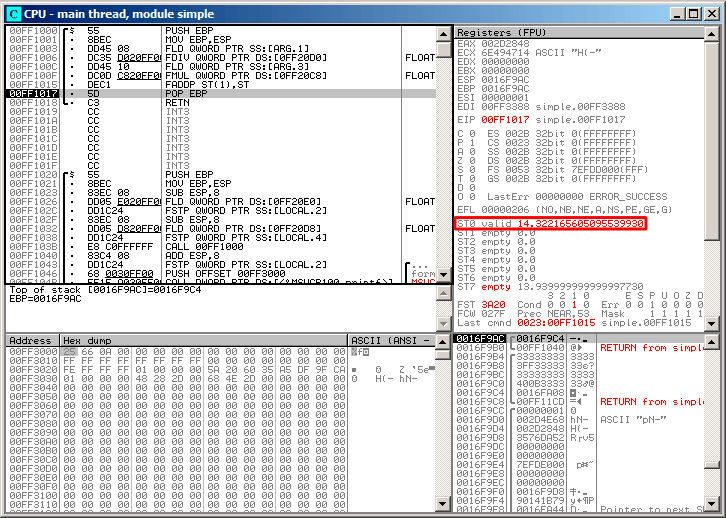
\includegraphics[scale=\FigScale]{patterns/12_FPU/1_simple/olly5.png}
\caption{\olly: \FADDP \RU{исполнилась}\EN{executed}}
\label{fig:FPU_simple_olly_5}
\end{figure}

\RU{Сумма остается в \ST{0} потому что функция возвращает результат своей работы через \ST{0}.}
\EN{The result is left in \ST{0}, because the function returns its value in \ST{0}.}
\RU{Позже \main возьмет это значение оттуда.}
\EN{\main takes this value from the register later.}

\RU{Мы также видим кое-что необычное: значение 13,93\ldots теперь находится в \ST{7}.}
\EN{We also see something unusual: the 13.93\ldots value is now located in \ST{7}.}
\RU{Почему}\EN{Why}?

\label{FPU_is_rather_circular_buffer}
\RU{Мы читали в этой книге, что регистры в \ac{FPU} представляют собой стек}
\EN{As we have read some time before in this book, the \ac{FPU} registers are a stack}: \myref{FPU_is_stack}. 
\RU{Но это упрощение}\EN{But this is a simplification}.
\RU{Представьте, если бы \IT{в железе} было бы так, как описано. Тогда при каждом заталкивании 
(или выталкивании) в стек,
все остальные 7 значений нужно было бы передвигать (или копировать) в соседние регистры, 
а это слишком много работы.}
\EN{Imagine if it was implemented \IT{in hardware} as it's described, 
then all 7 register's
contents must be moved (or copied) to adjacent registers during pushing and popping, 
and that's a lot of work.}
\RU{Так что в реальности у
\ac{FPU} есть просто 8 регистров и указатель (называемый \TT{TOP}), содержащий номер регистра,
который в текущий момент является \q{вершиной стека}.}
\EN{In reality, the \ac{FPU} has just 8 registers and a pointer (called \TT{TOP}) which contains a register number,
which is the current \q{top of stack}.}
\RU{При заталкивании значения в стек регистр \TT{TOP} меняется, и указывает на свободный регистр. 
Затем значение записывается в этот регистр.}
\EN{When a value is pushed to the stack, \TT{TOP} is pointed to the next available register,
and then a value is written to that register.}
\RU{При выталкивании значения из стека процедура обратная. Однако освобожденный регистр не обнуляется}
\EN{The procedure is reversed if a value is popped, however, the register which was freed is not cleared}
(\RU{наверное, можно было бы сделать, чтобы обнулялся, но это лишняя работа и работало бы медленнее}\EN{it 
could possibly be cleared, but this is more work which can degrade performance}).
\RU{Так что это мы здесь и видим}\EN{So that's what we see here}. 
\RU{Можно сказать, что \FADDP сохранила сумму, а затем вытолкнула один элемент.}
\EN{It can be said that \FADDP saved the sum in the stack, and then popped one element.}
\RU{Но в реальности, эта инструкция сохранила сумму и затем передвинула регистр \TT{TOP}.}
\EN{But in fact, this instruction saved the sum and then shifted \TT{TOP}.}
\RU{Было бы ещё точнее сказать, что регистры \ac{FPU} представляют собой кольцевой буфер.}
\EN{More precisely, the registers of the \ac{FPU} are a circular buffer.}

\fi
